\documentclass{article}

\usepackage{amsmath, amsfonts, microtype, xcolor, tikz, graphicx, hyperref, amsthm}
\usepackage[ruled, linesnumbered]{algorithm2e}
\usepackage[]{neurips_2019}
\newtheorem{theorem}{Theorem}


\title{Measuring causal influence with\\ back-to-back regression: the linear case - supplementary material}

\begin{document}

\appendix

\maketitle


\section{Theorem - detailed proof}
\label{sec:theorem}

\begin{theorem}[B2B consistency - general case]

     Consider the B2B model from Equation $$Y = (XE + N)F$$ $N$ centred and full rank noise.

     If $F$ and $X$ are full-rank on $Img(E)$, then, the solution of B2B, $\hat H$, will minimise

     $$\min_H  \left \| X - XH\right\| ^2  + \left \| NH\right \| ^2$$ and satisfy

     $$E\hat H = \hat H$$
\end{theorem}
\begin{proof}

 Let $\hat G$ and $\hat H$ be the solutions of the first and second regressions of B2B.

 Since $\hat G$ is the least square estimator of $X$ from $Y$
 \begin{align*}
    \hat G = \arg \min_G \mathbb{E}[\left \| YG - X \right \|^2]
\end{align*}
Replacing $Y$ by its model definition $Y = (XE+N)F$, we have
 \begin{align*}
    \hat G &=   \arg \min_G \mathbb{E}[\left \| X - (XE + N)FG \right\|^2] =\arg \min_G \mathbb{E}[\left \| X - XEFG + NFG \right\|^2]
  \end{align*}
  Since $N$ is centered and independent of $X$, we have
  \begin{align}
    	  \hat G &=  \arg \min_G \left \| X - XEFG\right\| ^2  + \left \| NFG\right \| ^2
     \label{eq:Gdoublenorm}
\end{align}

Samely, for $\hat H$, we have
\begin{align*}
    \hat H = \arg \min_H \mathbb{E}[\| XH - Y \hat{G} \|^2] &=\arg  \min_H \mathbb{E}[\| XH - (XE + N)F \hat G \|^2] \\
    &=\arg \min_H \mathbb{E}[\| X(H - EF \hat G) \| ^2] + \mathbb{E}[\| NF\hat G \| ^2]\\
    &= \arg \min_H \mathbb{E}[\| X(H - EF \hat G) \| ^2]
 \end{align*}
 a positive quantity which reaches a minimum (zero) for
 \begin{align}
    \hat H = EF \hat G
    \label{eq:Hdoublenom}
\end{align}

Let us now prove that $EF\hat G = F\hat G$.

Let $F^\dagger$ be the pseudo inverse of $F$, and $Z=F^\dagger EF\hat G$, we have $FZ = FF^\dagger EF \hat G$

Since $F$ is full rank on $Img(E)$, we have $FF^\dagger E =E$, and $FZ = EF\hat G$

As $E$ is a binary diagonal matrix, it is an orthogonal projection and therefore a contraction, thus
 $$ \| NEF\hat G\|^2 \leq \| NF\hat G \|^2$$ and
 $$\left \| X - XEFZ\right \| ^2  + \left \| NFZ\right \| ^2 = \| X - XEF\hat G \| ^2  + \| NEF\hat G \| ^2 \leq \| X - XEF\hat G \| ^2  + \| NF\hat G \| ^2$$

But since $\hat G =  \arg \min_G \left \| X - XEFG\right\| ^2  + \left \| NFG\right \| ^2$, we also have
$$\left \| X - XEF\hat G\right\| ^2  + \left \| NF\hat G\right \| ^2 \leq \left \| X - XEFZ\right \| ^2  + \left \| NFZ\right \| ^2$$

Summarizing the above,
$$\left \| X - XEF\hat G\right\| ^2  + \left \| NF\hat G\right \| ^2 \leq \| X - XEF\hat G \| ^2  + \| NEF\hat G \| ^2 \leq \| X - XEF\hat G \| ^2  + \| NF\hat G \| ^2$$
$$\left \| X - XEF\hat G\right\| ^2  + \left \| NF\hat G\right \| ^2 = \| X - XEF\hat G \| ^2  + \| NEF\hat G \| ^2$$
$$\left \| NF\hat G\right \| ^2 =  \| NEF\hat G \| ^2$$

$N$ being full rank, this yields $EF\hat G = F\Hat G$.

Replacing into $\eqref{eq:Gdoublenorm}$, and setting $H = EFG$, we have
\begin{align*}
	\hat G &=  \arg \min_G  \left \| X - XEFG\right \| ^2  + \left \| NFG\right \| ^2 \\
	&=   \arg \min_G \left \| X - XEFG\right \| ^2  + \left \| NEFG\right \| ^2 \\
	\hat H &=  \arg \min_H \left \| X - XH\right \| ^2  + \left \| NH\right \| ^2
	\label{eq:4}
\end{align*}

Finally, $E\hat H = E EF\hat G = EF\hat G = \hat H$, since $E$, a binary diagonal matrix, is involutive. This completes the proof.
\end{proof}



\section{Additional Figures}


\begin{figure}[t!]
  \centering
  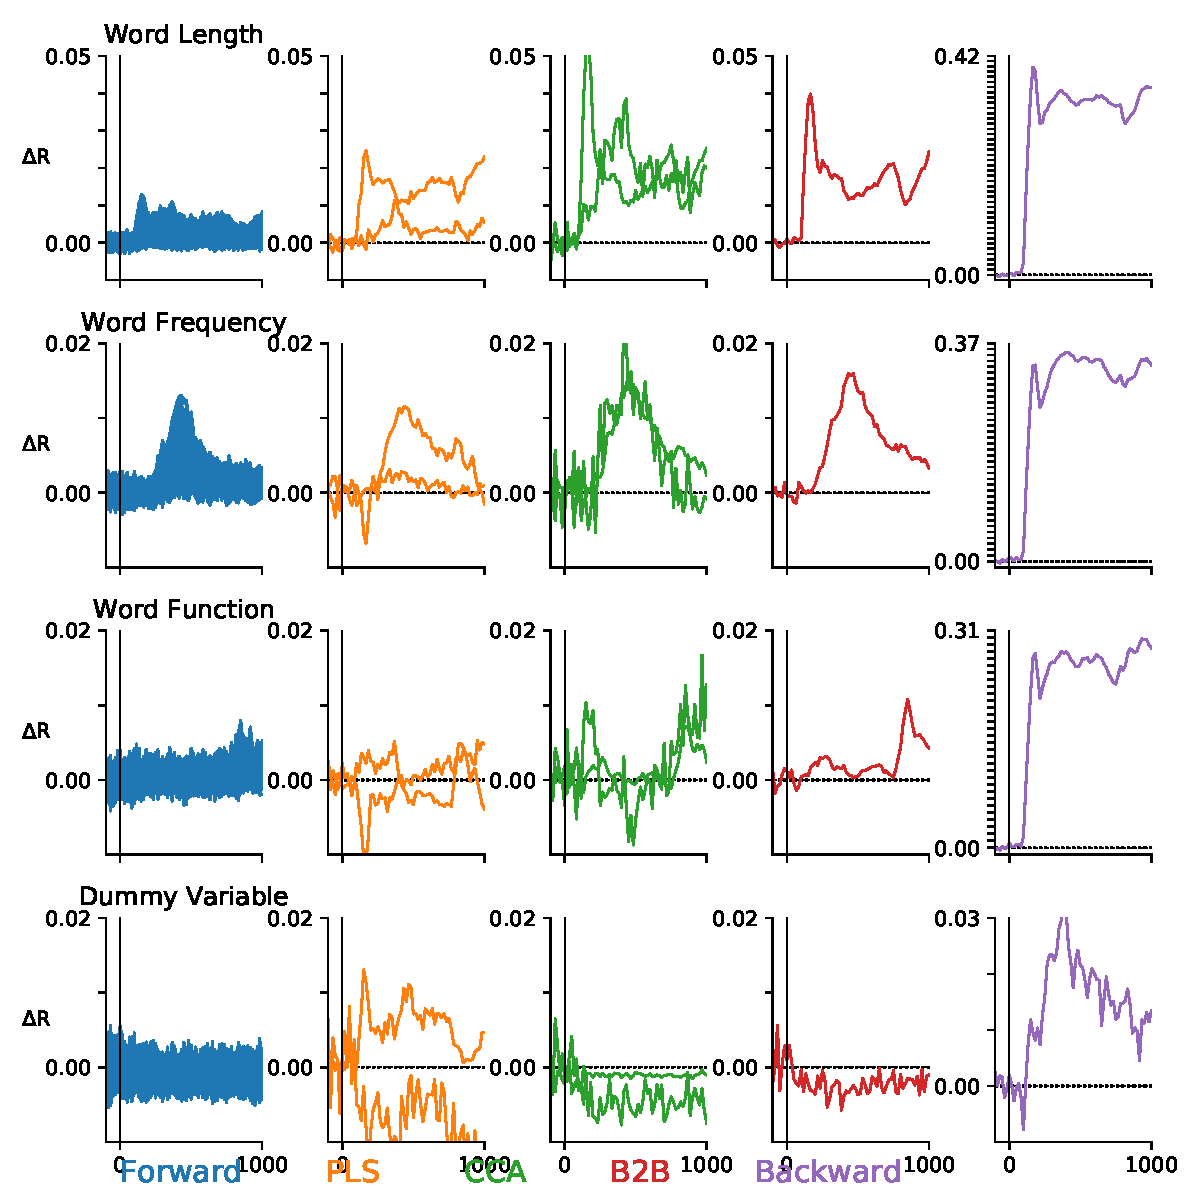
\includegraphics[width=\textwidth, trim=0cm 0cm 0cm 0cm, clip=True]{figures/meg_supp.pdf}
  \caption{}
  \label{fig:meg_supp}
\end{figure}

\end{document}
